\documentclass[10pt,a4paper]{article}
\usepackage[margin=0.6in, top=0.55in, bottom=0.55in]{geometry}
\usepackage{lmodern}
\usepackage[utf8]{inputenc}
\usepackage[T1]{fontenc}
\usepackage{booktabs}
\usepackage{tabularx}
\usepackage{xcolor}
\usepackage{graphicx}
\usepackage{amsmath}
\usepackage[colorlinks=true, linkcolor=blue!70!black, urlcolor=blue!70!black]{hyperref}

\setlength{\parskip}{2.5pt}
\setlength{\parindent}{0pt}

\begin{document}

% COVER PAGE
\begin{titlepage}
    \vspace*{4.0cm}
    \begin{center}
        {\Large\bfseries Information Visualization}\\[1.6em]
        {\huge\bfseries TMDB Movie Dashboard Project}\\[0.8em]
        {\large\bfseries Mini-Project 2: Interactive Dashboard}\\[0.4em]
        {\normalsize Week 5: Proposal + Sketches}
    \end{center}

    \vspace{5.0cm}
    \begin{flushleft}
    \setlength{\tabcolsep}{12pt}
    \renewcommand{\arraystretch}{1.4}
    \begin{tabular}{ll}
        \textbf{Full name:} & Satvik Boppudi \\
        \textbf{Date of submission:} & 14 October 2026 \\
        \textbf{Course name:} & Information Visualization \\
        \textbf{Instructor:} & Raz Saremi \\
        \textbf{Assignment title:} & Mini-Project 2: Interactive Dashboard \\
        \textbf{Collaborators:} & None \\
    \end{tabular}
    \end{flushleft}
    \vspace*{2.0cm}
\end{titlepage}

% BODY: PROPOSAL & SKETCHES
\begin{center}
    {\Large\bfseries MINI-PROJECT 2: INTERACTIVE DASHBOARD}\\[0.2em]
    {\normalsize\bfseries Week 5: Proposal + Sketches}\\[0.4em]
    \hrule height 0.8pt
    \vspace{0.25em}
    \begin{tabular*}{\textwidth}{@{\extracolsep{\fill}}ll}
        \textbf{Student:} Satvik Boppudi & \textbf{Course:} Information Visualization \\
        \textbf{Instructor:} Raz Saremi & \textbf{Project:} TMDB Movie Financial \& Reception Dashboard \\
    \end{tabular*}
    \vspace{0.25em}
    \hrule height 0.8pt
\end{center}

\vspace{0.2em}

\section*{1. Dataset Choice}

\textbf{Dataset:} \textbf{TMDB 5000 Movies Dataset} (Source: Kaggle via The Movie Database API; \url{https://www.kaggle.com/datasets/tmdb/tmdb-movie-metadata}).

\textbf{Rationale:} Film economics represents a compelling visual domain because massive capital investments do not guarantee box office profitability or critical praise. Spanning 4,803 films from 1916 to 2017, this dataset enables exploring how budgets correlate with revenue, critical reception, popularity, and historical shifts across cinematic genres.

\textbf{Dimensions (Mixing Quantitative, Ordinal/Temporal, and Categorical):}
\begin{itemize}\setlength{\itemsep}{0.5pt}\setlength{\parskip}{0pt}\setlength{\parsep}{0pt}
    \item \textbf{Production Budget (\texttt{budget\_millions}):} Quantitative (Continuous, \$0M to \$380M): Production expenditure in millions USD.
    \item \textbf{Box Office Revenue (\texttt{revenue\_millions}):} Quantitative (Continuous, \$0M to \$2,788M): Worldwide gross revenue in millions USD.
    \item \textbf{Popularity Score (\texttt{popularity}):} Quantitative (Continuous): TMDB algorithmic engagement metric.
    \item \textbf{Audience Vote Average (\texttt{vote\_average}):} Quantitative (Continuous Interval, 0.0 to 10.0): Audience rating average.
    \item \textbf{Release Year (\texttt{release\_year}):} Temporal / Ordinal (1916 to 2017): Year of theatrical release.
    \item \textbf{Primary Genre (\texttt{primary\_genre}):} Categorical / Nominal: Top 6 genres (Adventure, Action, Comedy, Drama, Horror, Crime) and ``Other''.
    \item \textbf{Movie Count (\texttt{movie\_count}):} Quantitative (Discrete): Frequency count of movies within rating intervals.
\end{itemize}

\section*{2. Three Research Questions}

\begin{enumerate}\setlength{\itemsep}{1.5pt}\setlength{\parskip}{0pt}\setlength{\parsep}{0pt}
    \item[\textbf{RQ1:}] \textbf{Financial Scale, Return, and Critical Acclaim:} How does a movie's production budget correlate with its worldwide box office revenue, and do higher-budget blockbuster productions reliably achieve superior audience ratings and popularity?
    \item[\textbf{RQ2:}] \textbf{Genre Profitability vs. Audience Sentiment:} Which primary movie genres produce the highest average box office return, and does high financial return align with favorable audience ratings?
    \item[\textbf{RQ3:}] \textbf{Cinematic Era Evolution and Rating Distributions:} How has average film revenue evolved across cinematic eras (from early cinema to the modern blockbuster era), and do release eras exhibit distinct audience rating profiles?
\end{enumerate}

\section*{3. Channel Justification Table}

\begin{center}
\footnotesize
\renewcommand{\arraystretch}{1.12}
\begin{tabularx}{\textwidth}{@{}l l l l p{2.2cm} X@{}}
\toprule
\textbf{Data Variable} & \textbf{Data Type} & \textbf{Mark} & \textbf{Channel} & \textbf{Principle} & \textbf{Justification} \\
\midrule
Budget (\$M) & Quantitative & Point & $X$-position & Effectiveness (Cleveland) & Position on common scale is Rank 1 for quantitative accuracy. \\
Revenue (\$M) & Quantitative & Point & $Y$-position & Effectiveness (Cleveland) & Position on common scale allows instant magnitude comparison. \\
Popularity & Quantitative & Point & Area (Circle size) & Stevens' Law ($\beta \approx 0.7$) & Perceived sub-linearly; secondary cue without dominating spatial axes. \\
Vote Average & Quantitative & Point & Color (Viridis) & Expressiveness \& Access. & Ordered continuous data on ordered lightness ramp; colorblind safe. \\
Primary Genre & Categorical & Bar & $Y$-position (Rows) & Expressiveness \& Legibility & Nominal categories mapped to discrete rows; labels read horizontally. \\
Avg Rev (Genre) & Quantitative & Bar & Length ($X$-axis) & Effectiveness (Cleveland) & Length on aligned scale allows rapid, pre-attentive comparison. \\
Release Year & Temporal & Line/Point & $X$-position & Convention \& Expressiveness & Cultural convention: time flows left to right. Line conveys continuity. \\
Avg Rev (Time) & Quantitative & Line vertex & $Y$-position & Effectiveness (Cleveland) & Vertical position on aligned scale traces historical revenue trajectory. \\
Vote Avg (Bins) & Quantitative & Bar & $X$-position & Expressiveness & Ordered 0.5-point intervals along horizontal axis show distribution shape. \\
Movie Count & Quantitative & Bar & Height ($Y$-axis) & Effectiveness (Cleveland) & Bar height on common baseline allows accurate frequency comparison. \\
\bottomrule
\end{tabularx}
\end{center}

\newpage

\section*{4. Wireframe Sketches of Dashboard Layout}

Below is the wireframe layout sketch for the interactive dashboard, illustrating the global filters panel, summary KPI overview cards, and the four coordinated views (Scatter Plot, Genre Bar Chart, Timeline Line Chart, and Rating Histogram):

\vspace{0.6em}
\begin{center}
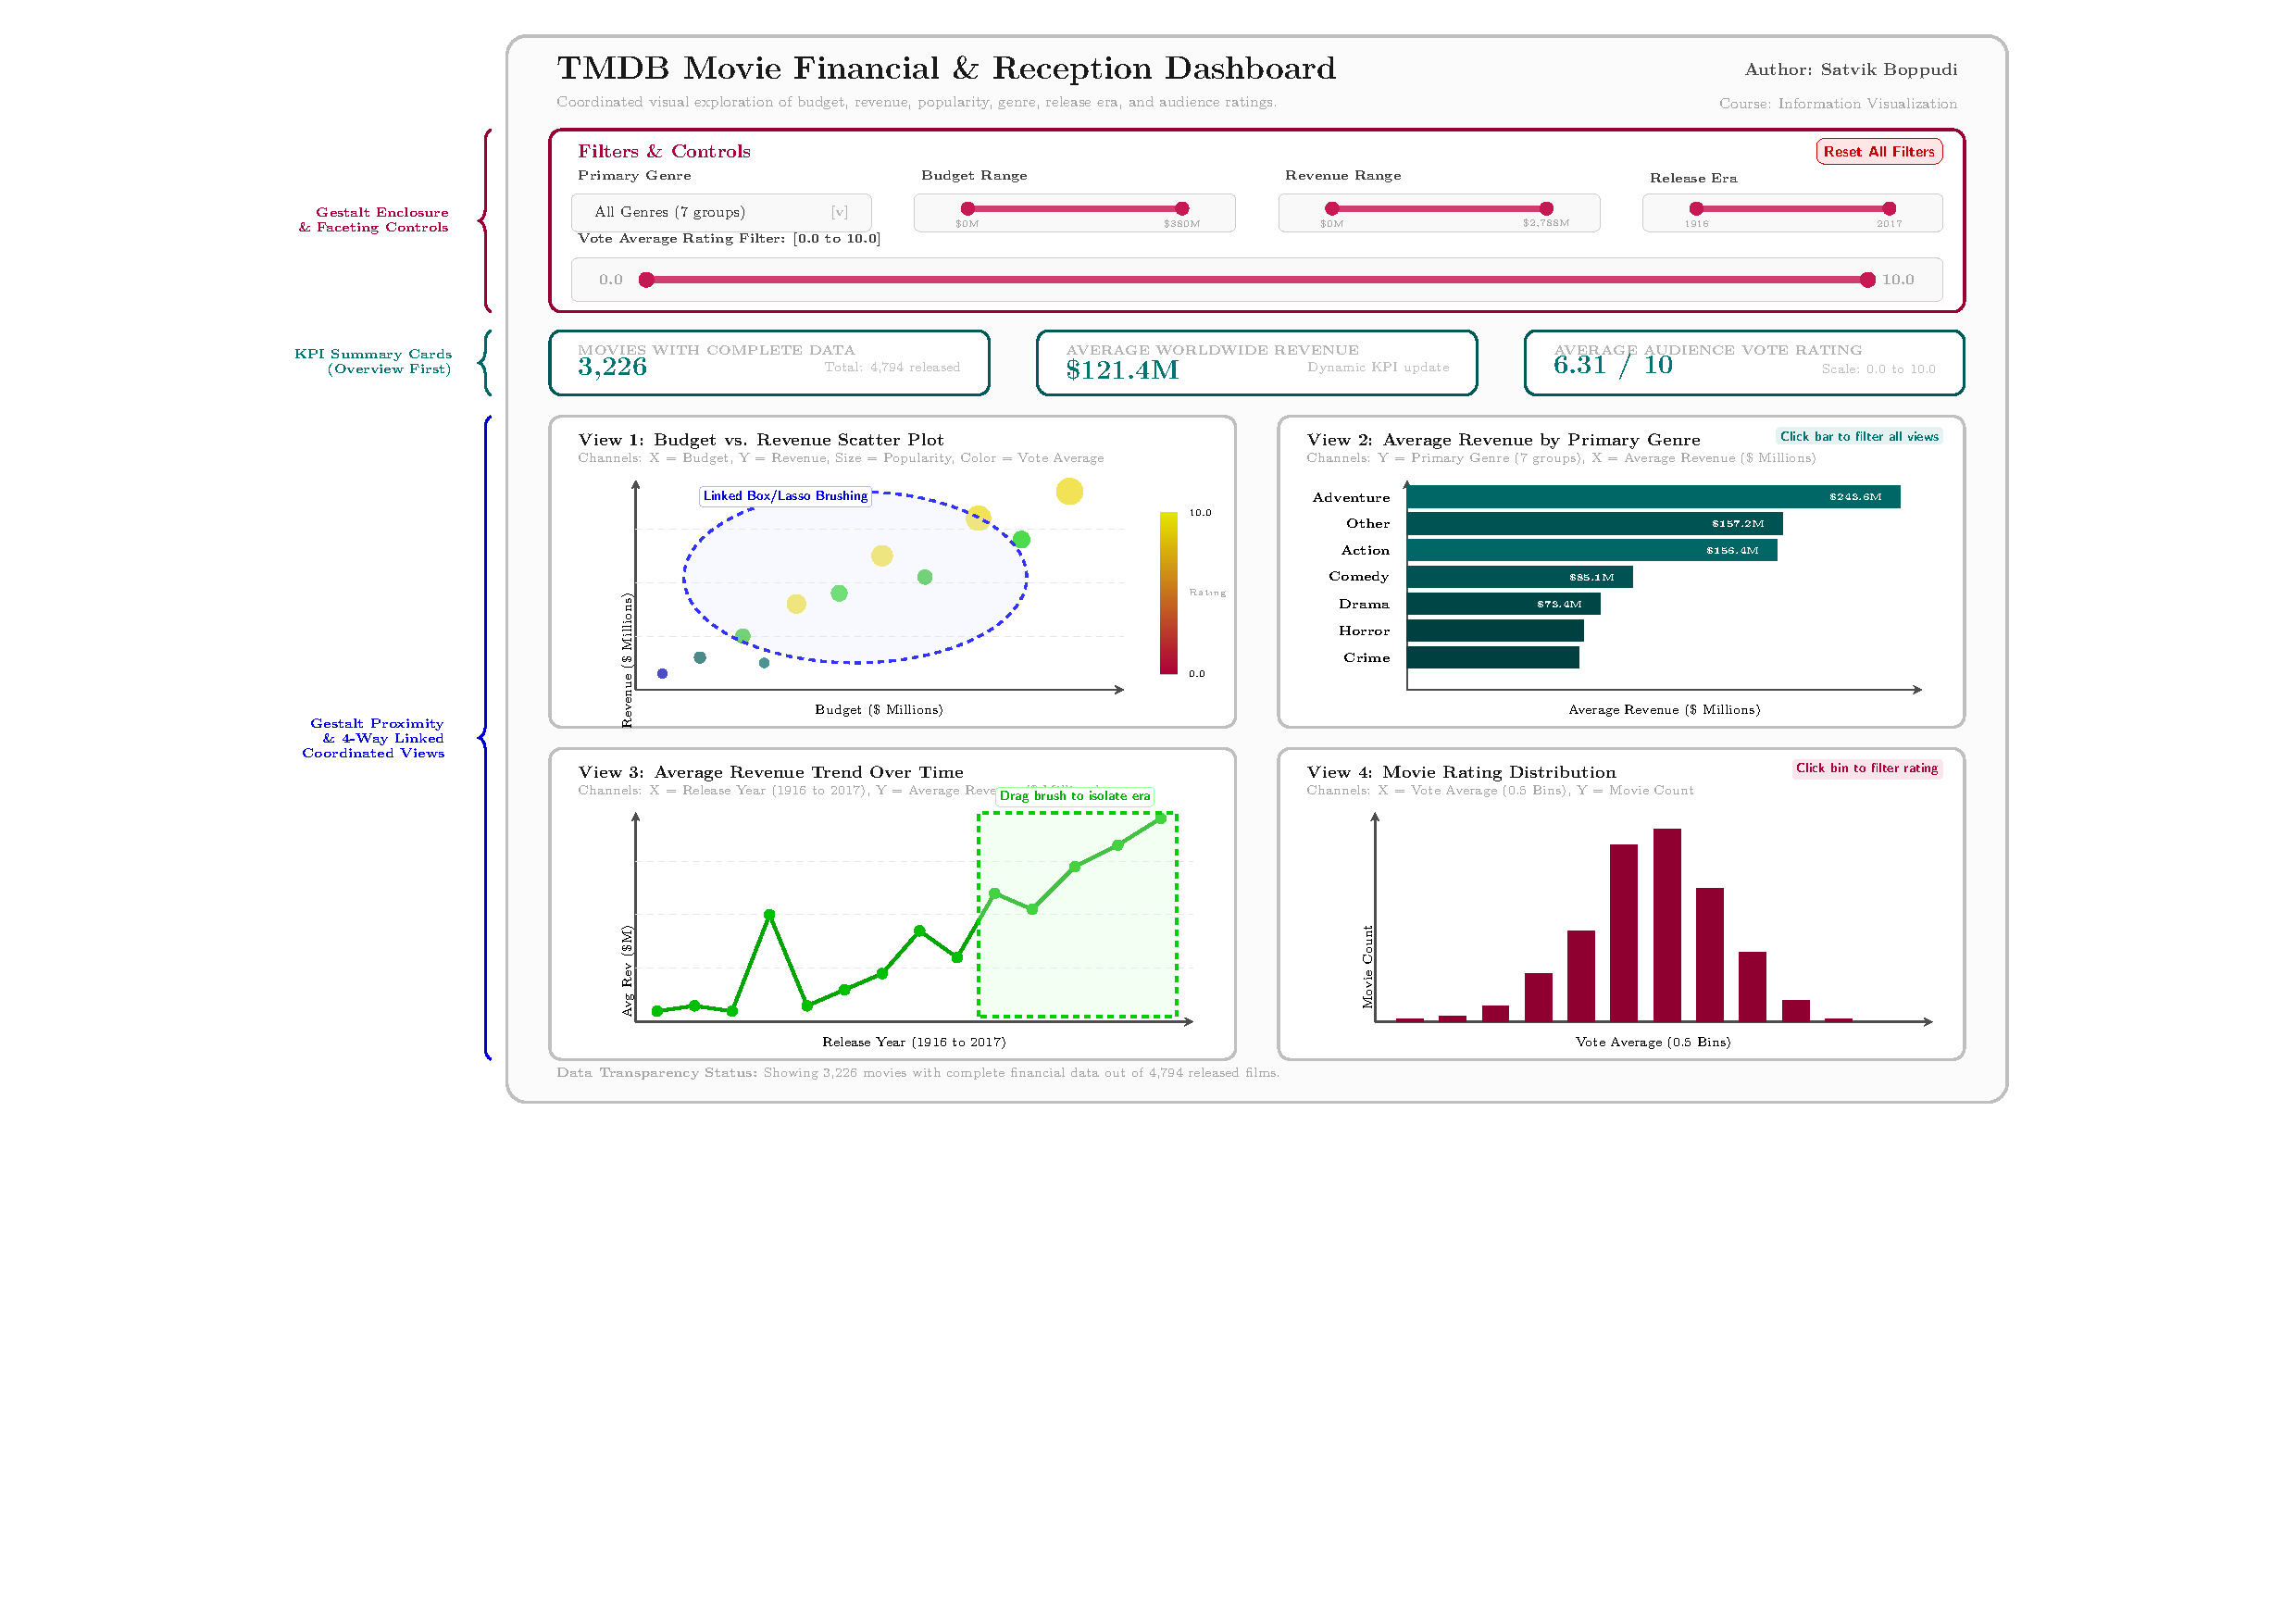
\includegraphics[width=\textwidth, height=0.88\textheight, keepaspectratio]{sketches/wireframe_selected_layout.pdf}
\end{center}

\end{document}
